% Copyright (C) 2012 Shi.Zhan <g.shizhan.g@gmail.com>
%
% Permission is hereby granted, free of charge, to any person obtaining a copy of this software and associated documentation files (the "Software"), to deal in the Software without restriction, including without limitation the rights to use, copy, modify, merge, publish, distribute, sublicense, and/or sell copies of the Software, and to permit persons to whom the Software is furnished to do so, subject to the following conditions:
%
% The above copyright notice and this permission notice shall be included in all copies or substantial portions of the Software.
%
% THE SOFTWARE IS PROVIDED "AS IS", WITHOUT WARRANTY OF ANY KIND, EXPRESS OR IMPLIED, INCLUDING BUT NOT LIMITED TO THE WARRANTIES OF MERCHANTABILITY, FITNESS FOR A PARTICULAR PURPOSE AND NONINFRINGEMENT. IN NO EVENT SHALL THE AUTHORS OR COPYRIGHT HOLDERS BE LIABLE FOR ANY CLAIM, DAMAGES OR OTHER LIABILITY, WHETHER IN AN ACTION OF CONTRACT, TORT OR OTHERWISE, ARISING FROM, OUT OF OR IN CONNECTION WITH THE SOFTWARE OR THE USE OR OTHER DEALINGS IN THE SOFTWARE.
%
% 课程:人机交互技术及应用
% 班级:传播学1001班
% 课时:40学时,2012年秋季1~10周,每周一、三
% 地点:东九楼D212
% 主页:http://code.google.com/p/hci-course/
% 教师:施展 
% 单位:华中科技大学 武汉光电国家实验室
%
\documentclass{beamer}
\usepackage{fontspec,xunicode,xltxtra,beamerthemesplit}
%\usetheme{Hannover} % White background
\usetheme{Berkeley} % Blue background
\setsansfont[Mapping=tex-text, ItalicFont={Courier Italic}]{Microsoft YaHei}

% 中文环境自动换行
\XeTeXlinebreaklocale "zh"
\XeTeXlinebreakskip = 0pt plus 1pt

% 中文环境修正导航栏
\makeatletter
\def\beamer@linkspace#1{%
  \begin{pgfpicture}{0pt}{-1.5pt}{#1}{5.5pt}
    \pgfsetfillopacity{0}
    \pgftext[x=0pt,y=-1.5pt]{.}
    \pgftext[x=#1,y=5.5pt]{.}
  \end{pgfpicture}}
\makeatother

\title{人机交互技术}
\author{施展}
\institute{华中科技大学~武汉光电国家实验室}
\date{\today}
\titlegraphic{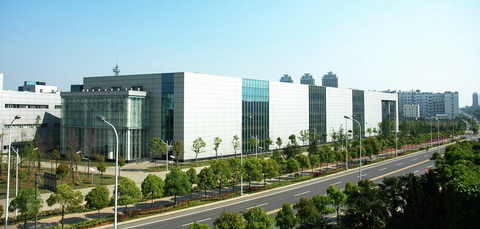
\includegraphics[width=3.5cm]{images/wnlo.jpg}}

\begin{document}

\begin{frame}
	\titlepage
\end{frame}

\begin{frame}
	\frametitle{内容提要}
	\tableofcontents
\end{frame}

\section{第二讲}
\begin{frame}
	\frametitle{第二讲 感知和认知基础}
	\begin{itemize}
		\item 人的感知
		\item 认知过程与交互设计原则
		\item 概念模型及认知
		\item 分布式认知
	\end{itemize}
\end{frame}

\subsection{人的感知}
\begin{frame}
	\frametitle{人的感知}
	\beamertemplatetransparentcovereddynamicmedium 
	\begin{itemize}[<+->]
		\item 人的感知即通过人体器官和组织进行人与外部世界的信息的交流和传递
		\item 认知是人们在进行日常活动时发生于头脑中的事情
		\begin{itemize}
			\item 涉及思维、记忆、学习、幻想、决策、看、读、写和交谈等
		\end{itemize}
		\item 人的感知是认知的基础,认知是将感知获取的信息综合运用
		\begin{itemize}
			\item 认知分为经验认知和思维认知
			\item 认知过程是相互联系的,单纯的一个认知过程是非常少见的
		\end{itemize}
	\end{itemize}
\end{frame}

\begin{frame}
	\frametitle{认知心理学 Cognitive Psychology}
	\beamertemplatetransparentcovereddynamicmedium 
	\begin{itemize}
		\item 认知心理学是二十世纪50年代中期在西方兴起的一种心理学思潮,二十世纪70年代开始其成为西方心理学的一个主要研究方向。
		\pause
		\item 是作为人类行为基础的心理机制,其核心是输入和输出之间发生的内部心理过程。
		\pause
		\item 与西方传统哲学也有一定联系,其主要特点是强调知识的作用,认为知识是决定人类行为的主要因素。
		\pause
		\item 认知心理学研究:
		\begin{itemize}
			\item 人们如何获得外部世界信息
			\item 信息在人脑内如何表示并转化为知识
			\item 知识怎样存储又如何用来指导人们的注意和行为
		\end{itemize}
	\end{itemize}
\end{frame}

\begin{frame}
	\frametitle{感知通道}
	\beamertemplatetransparentcovereddynamicmedium 
	\begin{itemize}[<+->]
		\item 五种基本感知的绝对阈限:
		\begin{itemize}
			\item 视觉: 在黑暗而空气清新的夜晚, 人们可以看到30 英里( 48000 千米) 外的一只烛光( 1 英里≈1.6 千米) ; 
			\item 听觉: 在安静的环境中, 人能够听到20英尺远处的手表滴答声( 1 英尺= 0.3 米) ; 
			\item 嗅觉: 人能嗅到1 公升空气中散布的1/10 万毫克的人造麝香的气味; 
			\item 味觉: 人可尝出9 升水中放一茶匙糖的甜味; 
			\item 触觉: 人可感到蜂蜜翅膀距脸颊1 厘米处落下。
		\end{itemize}
	\end{itemize}
\end{frame}

\subsection{认知过程与交互设计原则}
\begin{frame}
	\frametitle{认知过程与交互设计原则}

\end{frame}

\subsection{概念模型及认知}
\begin{frame}
	\frametitle{概念模型及认知}

\end{frame}

\subsection{分布式认知}
\begin{frame}
	\frametitle{分布式认知}

\end{frame}

\section{小结}
\begin{frame}
	\frametitle{小结}
	\begin{itemize}
		\item 了解人的感知模型
		\item 掌握认知过程与交互设计原则
		\item 掌握概念模型及对概念模型的认知
		\item 了解分布式认知
	\end{itemize}
\end{frame}
 
\end{document}